\documentclass[a4paper,12pt,twoside]{report}
\usepackage[left=3cm,right=3cm,top=2cm,bottom=3cm]{geometry}
%\usepackage[square,authoryear,sort]{natbib}
\usepackage{url}
\usepackage{xcolor}
\usepackage{graphicx}
\usepackage{pdfpages}
\usepackage{subcaption}
%\usepackage{pgfgantt}
\usepackage{dirtytalk}

\makeatletter
\def\@makechapterhead#1{%
  \vspace*{50\p@}%
  {\parindent \z@ \raggedright \normalfont
    \interlinepenalty\@M
    \Huge\bfseries  \thechapter.\quad #1\par\nobreak
    \vskip 40\p@
  }}
\makeatother

\makeatletter
\newcommand*{\toccontents}{\@starttoc{toc}}
\makeatother

\newtheorem{hypothesis}{Hypothesis}

\newtheorem{rquestion}{Research Question}


\let\endtitlepage\relax
\begin{document}

\title{\LARGE {\bf Progress Report: Henry Clausen}\\
 \vspace*{-5mm}
}
\author{Henry Clausen}
%\date{October 2008}

\maketitle



\toccontents
%\begin{abstract}
%Text
%\end{abstract}



\chapter{Short-term contextual model of network flows using LSTM networks}

In the context of the overall research goal of this project, some exploratory work on contextual anomaly detection for network events was conducted before my PhD started by Marc Sabate, Gudmund Grov, Wei Chen, and David Aspinall. 
This work uses a recurrent neural network to capture meaningful sequences of \textit{NetFlows} and reflect reccurring patterns in a model. For that, recorded NetFlows are grouped according to the generating host. Furthermore, to filter out sequences of flows that are unrelated to each other, a squence of flows that are close in time is grouped into what is called a \say{session} as an approximation of the true relation. Each session then serves as a training or test sequence for a behavioural model. Learned semantic behaviour is reflected through the capability of the model to predict traffic protocols and network ports of flows in a session from a smaller subset of flows, with more accurate predictions being rewarded in the training process. Sessions which deviate from previously observed behaviour are then predicted poorly by the model and flagged as potentially malicious.

This work however was not yet complete for successful publication, \textcolor{red}{which is why I took the responsibilty to bring it to a state of ...}. During my work, I made significant changes and additions to both improve the model performance as well as extend the evaluation to highlight the benefits and novelty of this work. 
In particular, I made the following major changes:

\begin{enumerate}
\item I specified the scope of the model to the detection of U2R and R2L attacks, to which it is more suited than high volume attacks. I also exchanged the evaluation datasets to mutiple ones that are more suitable for this task and more realistic in nature.
\item Originally, the model only incorporated the protocol and the port for each flow. I extended this to the direction (from or to host) as well as the size of each flow, which improved detection rates especially for brute-force attacks and sql injections. For this, I came up with an efficient way to process these additional inputs without significant increase of model size.
\item Similarly, the original model was a standard recurrent neural network with one layer. I extended this to a bidirectional LSTM network with multiple layers, which required careful parameter calibration and further boosted detection rates.
\item The detection method was changed from an overall host classification to a session classification using a scoring threshold, which is more realistic in a real-world deployment due to the high imbalance between benign and malicious traffic.
\item I carfed out the novelty and contribution of this work more, and implemented three comparision benchmark models to highlight the benefit of our model. I also highlighted the differences between our work and recent applications of LSTMs to intrusion detection.
\end{enumerate}

\begin{figure}
\centering
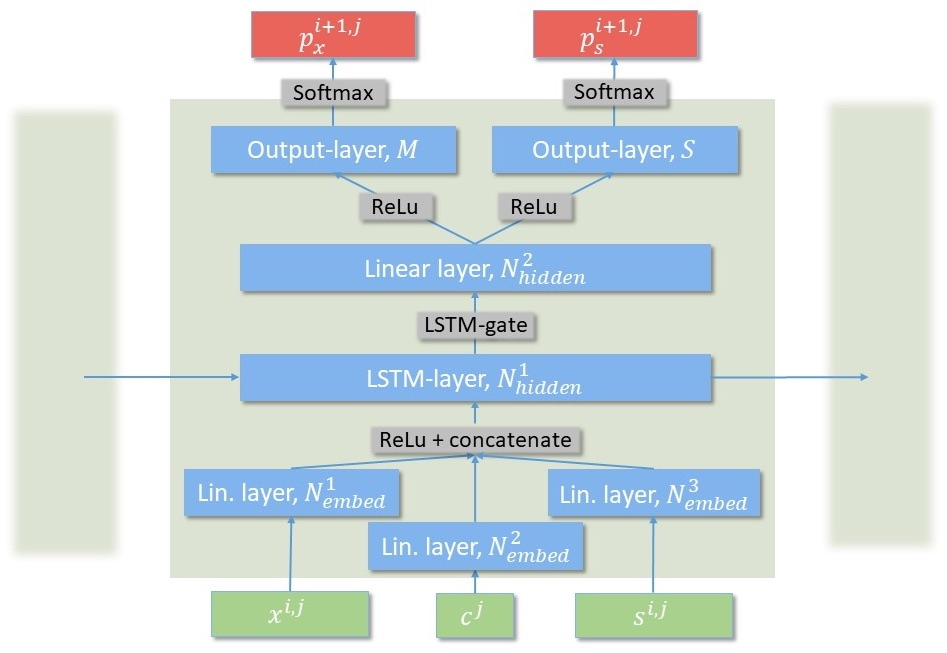
\includegraphics[width=0.7\textwidth]{images/LSTM_design_new2.jpg}
\caption{Bla}
\label{fig:LSTM}
\end{figure}

Since the paper is now in under my responsibility, and due to all the efforts I put into its improvement, we agreed that I would be the first author of this work in the event of publication. 

\textcolor{red}{difficulties}
\cite{sommer_outside_2010}

\chapter{Traffic Generation using Containerization for Machine Learning}

Building contextual models of network traffic means to build an understanding how different network interactions can be distinguished via their traffic trace. However, available network traffic datasets do not contain ground truth labels about the nature of computer interactions and often suffer from a lack of realism. To improve this and ensure that our models extract meaningful sets of sequences that represent these different interactions, we started developing a containerised traffic generation framework to generate traffic with ground truth labels. 

%Network traffic datasets are already hard to obtain due to privacy concerns. However, as  the correspondence between individual network traffic events and their particular purpose is virtually never recorded on a computer, very few datasets contain ground truth about the captured events. For that reason, a particular aspect of this project is to generate useful ground truth data with appropriate content myself.

This framework generates controlled and isolated network traffic from a variety of applications and tasks. For this, a virtual network was created using the virtualisation program \textit{Docker}. In this network, two or more parties can communicate through containers,  which are sandboxes containing programs inside a minimal virtualised operating system. The benefit of this design is that individual containers can only communicate with each other via the virtualised network while the host is in complete control of the parallel execution of tasks in multiple containers. To capture the traffic, every container in the network was complemented with a \textit{tcpdump}\footnote{A common packet capture utility} container hooked onto the network interface. The captured traffic can then be labelled according to the particular scenario it was generated by. We implemented a variety of network service  scenarios to capture a diverse set of network traffic.

\begin{figure}
\centering
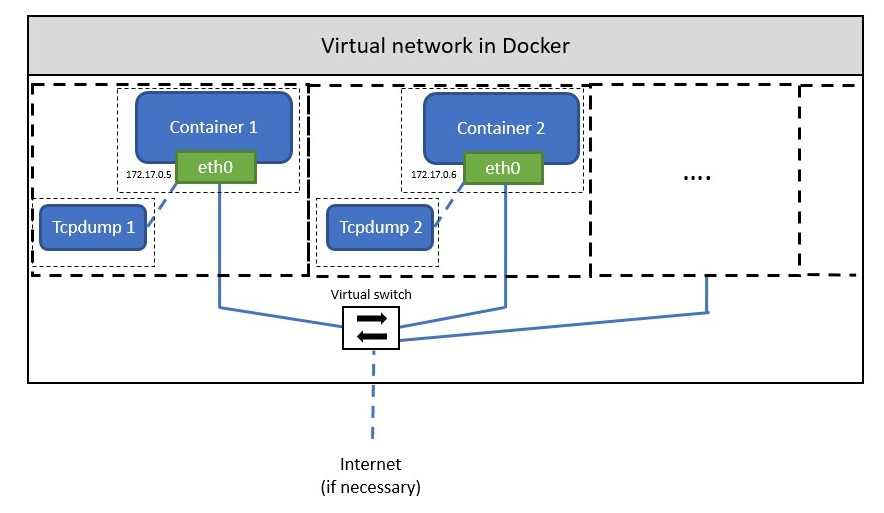
\includegraphics[width=0.7\textwidth]{images/Dockernet.jpg}
\caption{Visualisation of the virtual network in Docker}\label{docker}
\end{figure}


We emphasised the following particular strengths in our framework, which makes the generated data particularly suitable for ML-applications:
\begin{itemize}
\item traffic variation through a diversity of generation scenarios as well as transmission disturbances,
\item ground truth labels through containerised separation of generation scenarios,
\item scalability of the amount of generated traffic,
\item and modularity of the framework to easily extend and update the set of scenarios.
\end{itemize}



This work was started in summer 2018 by me and Nikola Pavlov\footnote{an LFCS summer intern}, and continued in summer 2019 by me and Robert Flood\footnote{an LFCS MSc student}. My responsibilities lied in overall design of the framework as well as the requirements on the generation features, testing and extending individual scenarios as well as implemention, and the design and conduction of validation experiments. 

In autumn of 2019, Robert Flood and I described the framework in a paper of which I am first author, which was submitted and accepted at the ACSAC DYNAMICS workshop 2019, and will appear in the corresponding proceedings this March. 

Due to very positive feedback at the workshop as well as encouragements and suggestions to extend the framework, we are working further on this project, which is described in Section \textcolor{red}{.....}

\section{1. stint at BT - Stepping stone detection and connection correlation}

As part of my CASE PhD scholarship, I spent six weeks with my industrial sponsor at BT Labs Adastral Park in August and September 2019. Before starting this stint, I met with my industrial supervisors to define a project to work on that is both related to my PhD and is a relevant problem for BT. During this meeting, we agreed that the problem of detecting stepping stones



\section{Modelling of connection establishment via LSTM encoders}

\section{Problems with publishing in Network Anomaly Detection}

\section{Future plans}

%\section{Introduction and motivation}







%\addcontentsline{toc}{section}{Bibliography}
\bibliographystyle{abbrv}
\bibliography{refs}

\end{document}